\begin{name}
	{\tenchude}
	{TOÁN 10}
	{LỚP TOÁN THẦY PHÁT}
	{Life isn’t about finding yourself. Life is about creating yourself}
\end{name}
\Opensolutionfile{ansbook}[ans/ansbookDe4]
\TN
\Opensolutionfile{ans}[ans/ansDe4-TN1]
\begin{ex}%[0-TK-HK1-CT-6-2425]%[VN-MT-9, Phan Hoàng Anh]%[0D6N3-3]
Số điểm mà $5$ học sinh lớp 10A đạt được trong đợt thi đua học tập chào mừng ngày 20/11 như sau: $9$; $8$; $10$; $7$; $8$. Tìm số trung vị của mẫu số liệu trên.
\choice
{$7$}
{$10$}
{$9$}
{\True $8$}
\loigiai{Sắp xếp mẫu số liệu theo thứ tự không giảm như bên dưới
\[7\qquad8\qquad8\qquad9\qquad10.\]
Trung vị của mẫu số liệu là $M_{\text{e}}=8$.}
\end{ex}

\begin{ex}%[0D6N4-2]%[KNTT - Lớp 10 - Ôn tập cuối học kì 1 - Đề 6]%[Nguyễn Hoài Nam]
Mẫu số liệu sau đây cho biết cân nặng của $10$ trẻ sơ sinh (đơn vị kg)
\begin{center}
\begin{tabular}{ccccc}
$2{,}977$ & $3{,}155$ & $3{,}920$ & $3{,}412$ & $4{,}236$  \\
$2{,}593$&	$3{,}270$ & $3{,}813$ & $4{,}042$ & $3{,}387$      \\
\end{tabular}
\end{center}
Khoảng biến thiên của mẫu số liệu trên là
\choice
{$0{,}384$}
{$0{,}194$}
{\True $1{,}643$}
{$3$}
\loigiai{Trước hết, ta sẽ sắp xếp mẫu số liệu theo thứ tự không giảm:

\begin{center}
\begin{tabular}{cccccc}
$2{,}593$ & $2{,}977$ & $3{,}155$ & $3{,}270$ & $3{,}387$ & $3{,}412$ \\
$3{,}813$ & $3{,}920$ & $4{,}042$ & $4{,}236$ &       &       \\
\end{tabular}

\end{center}
Khoảng biến thiên là $R = 4{,}236 - 2{,}593 = 1{,}643$.
}
\end{ex}

\begin{ex}%[0D8H1-3]
Từ các chữ số $1$, $2$, $3$, $4$, $5$ có thể lập được bao nhiêu số tự nhiên bé hơn $60$?
\choice
{$42$}
{\True $30$}
{$25$}
{$17$}
\loigiai{
\begin{itemize}
\item Số cần tìm có $1$ chữ số $\Rightarrow$ có $5$ số thỏa mãn yêu cầu.
\item Số cần tìm có $2$ chữ số $\Rightarrow$ có $5\cdot 5=25$ số thỏa mãn yêu cầu.
\end{itemize}
Vậy có $5+25=30$ (số thỏa mãn yêu cầu).
}
\end{ex}

\begin{ex}%[0D8H2-3]
Có bao nhiêu số chẵn mà mỗi số có $ 4$ chữ số đôi một khác nhau?
\choice
{$ 2520$}
{$ 50000$}
{$ 4500$}
{\True $ 2296$}
\loigiai{
\begin{itemize}
\item Số có $ 4$ chữ số khác nhau đôi một: $ 9\cdot \mathrm{A}_9^3$.
\item Số có $ 4$ chữ số lẻ khác nhau đôi một: $ 5\cdot8\cdot\mathrm{A}_8^2$.
\end{itemize}
Vậy số có $ 4$ chữ số chẵn khác nhau đôi một: $ 9\cdot\mathrm{A}_9^3-5\cdot8\cdot\mathrm{A}_8^2=2296$.}
\end{ex}

\begin{ex}%[0D8H2-4]
Một nhóm học sinh có $6$ học sinh nam và $4$ học sinh nữ. Chọn ngẫu nhiên $2$ học sinh. Tính xác suất sao cho $2$ học sinh được chọn có cả nam và nữ.
\choice
{$\mathrm{P}(A)=\dfrac{1}{5}$}
{\True $\mathrm{P}(A)=\dfrac{8}{15}$}
{$\mathrm{P}(A)=\dfrac{2}{9}$}
{$\mathrm{P}(A)=\dfrac{4}{15}$}
\loigiai{
Số cách chọn 2 học sinh trong 10 học sinh là $ \mathrm{C}_{10}^2$.\\
Nên số phần tử của không gian mẫu là $ n\left(\Omega\right)=\mathrm{C}_{10}^2=45$.\\
Gọi $A$ là biến cố \lq\lq Hai học sinh được chọn có cả nam và nữ\rq\rq .\\
Khi đó theo quy tắc nhân, số phần tử của biến cố $ A$ là $ n(A)=\mathrm{C}_6^1\cdot\mathrm{C}_4^1=24$.\\
Vậy xác suất để chọn được hai học sinh có cả nam và nữ là $ \mathrm{P}(A)=\dfrac{n(A)}{n\left(\Omega\right)}=\dfrac{24}{45}=\dfrac{8}{15}$.}
\end{ex}

\begin{ex}%[0D8H2-6]
Cho tứ diện $ABCD$. Hỏi có bao nhiêu vectơ khác vectơ $\overrightarrow{0}$ mà mỗi vectơ có điểm đầu, điểm cuối là hai đỉnh của tứ diện $ABCD$?
\choice
{\True $12$}
{$4$}
{$10$}
{$8$}
\loigiai{
Ta có mỗi vectơ khác vectơ $\overrightarrow{0}$ có điểm đầu và điểm cuối là $2$ đỉnh trong số $4$ đỉnh của tứ diện là một chỉnh hợp chập $2$ của $4$ phần tử.\\
Vậy số vectơ khác vectơ $\overrightarrow{0}$ có điểm đầu, điểm cuối là hai đỉnh của tứ diện $ABCD$ là $\mathrm{A}_4^2=12$.}
\end{ex}

\begin{ex}%[0D8H3-2]
Khai triển của nhị thức ${\left( x-\dfrac{1}{x} \right)^5}$là
\choice
{$x^5+5x^3+10x+\dfrac{10}{x}+\dfrac{5}{x^3}+\dfrac{1}{x^5}$}
{\True $x^5-5x^3+10x-\dfrac{10}{x}+\dfrac{5}{x^3}-\dfrac{1}{x^5}$}
{$5x^5-10x^3+10x-\dfrac{10}{x}+\dfrac{5}{x^3}-\dfrac{1}{x^5}$}
{$5x^5+10x^3+10x+\dfrac{10}{x}+\dfrac{5}{x^3}+\dfrac{1}{x^5}$}
\loigiai{
Ta có ${\left( x-\dfrac{1}{x} \right)^5}=\mathrm{C}_5^0.x^5+\mathrm{C}_5^1.x^4.{{\left( \dfrac{-1}{x} \right)}^1}+\mathrm{C}_5^2x^3{{\left( \dfrac{-1}{x} \right)}^2}+\mathrm{C}_5^3x^2{{\left( \dfrac{-1}{x} \right)}^3}+\mathrm{C}_5^4x^1{{\left( \dfrac{-1}{x} \right)}^4}+\mathrm{C}_5^5{{\left( \dfrac{-1}{x} \right)}^5}=\text{ }{x^5}-5x^3+10x-\dfrac{10}{x}+\dfrac{5}{x^3}-\dfrac{1}{x^5}$.}
\end{ex}

\begin{ex}%[0H9H1-2]
Cho hai điểm $ A(1;0) $ và $ B(0;-2) $. Tọa độ điểm $ D $ thỏa mãn $ \vec{AD}=-3\vec{AB} $ là
\choice
{ $(4;-6) $}
{$ (2;0) $}
{$ (0;4)  $}
{\True$ (4;6)  $}
\loigiai{
Gọi $ D(x_D;y_D) $.\\
Ta có 	$ \vec{AD}=-3\vec{AB} \Leftrightarrow \heva{&x_D-1=-3(0-1)\\&y_D-0=-3(-2-0)}\Leftrightarrow \heva{&x_D=4\\&y_D=6.}$  Vậy $ D(4;6) $.
}
\end{ex}

\begin{ex}%[10-11-12EX-HK1-2425]%[Trương Quan Kía]%[0H9H3-2]
Đường thẳng đi qua điểm $A(1; 11)$ và song song với đường thẳng $3x - y + 5 = 0$ có phương trình là
\choice
{\True $3x - y + 8 = 0$}
{$3x - y - 14 = 0$}
{$x + 3y - 34 = 0$}
{$x + 3y - 14 = 0$}
\loigiai
{
Gọi $d$ là phương trình đường thẳng cần tìm.\\
$d\parallel 3x-y+5=0$ nên $d\colon 3x-y+m=0$ ($m\ne 5$).\\
$d$ đi qua $A(1;11)$ nên $3\cdot 1-11+m=0\Rightarrow m=8$ (nhận).\\
Vậy $d\colon 3x-y+8=0$.
}
\end{ex}

\begin{ex}%[0H9H4-2]%[Dự án đề kiểm tra Toán 10 HKII NH23-24- Trung Anh]%[THPT Việt Đức - Hà Nội]
Trong mặt phẳng với hệ trục tọa độ $Oxy$, đường tròn $(C)$ có tâm $I(1;-2)$ và tiếp xúc với trục $Ox$ có phương trình là
\choice
{$(C): (x+1)^2+(y-2)^2=1$}
{\True $(C): (x-1)^2+(y+2)^2=4$}
{$(C): (x-1)^2+(y+2)^2=1$}
{$(C): (x+1)^2+(y-2)^2=4$}
\loigiai{
Đường tròn $(C)$ có tâm $I(1;-2)$ và tiếp xúc với trục $Ox$ nên suy ra \[R=|-2|=2.\]
Đường tròn $(C)$ có phương trình là \[(x-1)^2+(y+2)^2=4.\]
}
\end{ex}

\begin{ex}%[soạn để GHK, HK]%[Huỳnh Xuân Tín]%[0H9H5-2]
Cho elip $(E)$ có một đỉnh $A_2(7;0)$, một tiêu điểm $F_2(5;0)$.  Lập phương trình chính tắc của $(E)$.
\choice
{\True $\dfrac{x^2}{49}+\dfrac{y^2}{24}=1$}
{$\dfrac{x^2}{24}+\dfrac{y^2}{49}=1$}
{$\dfrac{x^2}{49}+\dfrac{y^2}{25}=1$}
{$\dfrac{x^2}{49}-\dfrac{y^2}{24}=1$}
\loigiai{
Ta có đỉnh $A_2(7;0)$, một tiêu điểm $F_2(5;0)$, suy ra $a=7$,  $c=5$ và $b^2=a^2-c^2=24$, do đó  $\dfrac{x^2}{49}+\dfrac{y^2}{24}=1$.
}
\end{ex}

\begin{ex}%[0H9H5-4]%[Dự án đề kiểm tra Toán 10 GHKI NH23-24- Lam Nguyen]%[THPT Le Quý Đôn - TPHCM]
Cho đường hypebol có phương trình $(H): 9x^2-3y^2=1$. Khoảng cách giữa hai tiêu điểm của hypebol là
\choice
{$0$}
{$\dfrac{\sqrt{2}}{3}$}
{\True $\dfrac{4}{3}$}
{$\dfrac{2}{3}$}
\loigiai{
Phương trình chính tắc của hypebol $(H): \dfrac{x^2}{\tfrac{1}{9}}-\dfrac{y^2}{\tfrac{1}{3}}=1$.\\
Vậy ta có $a^2=\dfrac{1}{9}$, $b^2=\dfrac{1}{3}$.\\
$c^2=b^2+a^2=\dfrac{1}{3}+\dfrac{1}{9}=\dfrac{4}{9} \Rightarrow c=\dfrac{2}{3}$.\\
Vậy khoảng cách giữa hai tiêu điểm của hypebol là $2c=\dfrac{4}{3}$.

}
\end{ex}

\TNTF
\begin{ex}%[0D8H2-4]
Chọn $4$ trong số $3$ học sinh nam và $5$ học sinh nữ tham gia một cuộc thi. Khi đó
\choiceTF
{\True Nếu chọn $2$ nam và $2$ nữ thì có $30$ cách chọn}
{Nếu trong số học sinh được chọn nhất thiết phải có học sinh nam $A$ và học sinh nữ $B$ thì có $30$ cách chọn}
{\True Nếu phải có ít nhất một trong hai học sinh $A$ và $B$ được chọn, thì có $55$ cách chọn}
{Nếu trong $4$ học sinh được chọn phải có cả học sinh nam và học sinh nữ thì có $55$ cách chọn}
\loigiai{
\begin{itemchoice}
\itemch Đúng vì Chọn $2$ trong $3$ học sinh nam, rồi chọn $2$ trong $5$ học sinh nữ nên số cách chọn là $\mathrm{C}_3^2\cdot\mathrm{C}_5^2=30$.
\itemch Sai vì Sau khi đã có $A$ và $B$, chọn $2$ trong $6$ học sinh còn lại. Ta có $\mathrm{C}_6^2=15$ cách chọn.
\itemch Đúng vì Chia thành $3$ phương án: có cả $A$ và $B$; chỉ có $A$; chỉ có $B$.\\
Nên ta có $\mathrm{C}_6^2+\mathrm{C}_6^3+\mathrm{C}_6^3=15+20+20=55$ cách chọn.
\itemch Sai vì Chia thành $3$ phương án: có $1$ học sinh nam; có $2$ học sinh nam; có $3$ học sinh nam.\\
Nên ta có $\mathrm{C}_3^1\cdot\mathrm{C}_5^3+\mathrm{C}_3^2\cdot\mathrm{C}_5^2+\mathrm{C}_3^3\cdot\mathrm{C}_5^1=3\cdot 10+3\cdot 10+1\cdot 5=65$ cách chọn.
\end{itemchoice}
}
\end{ex}

\begin{ex}%[Dự án 18 - TeamTeXHoa - Phạm Quốc Toàn]%[0H9H4-5]
Cho đường thẳng $d \colon x-my-2=0$ và đường tròn $\left( C \right) \colon \left( x-3 \right)^{2}+\left( y-1 \right)^{2}=4$. Các khẳng định sau đúng hay sai?
\choiceTF
{Với $m=2$ thì $d$ và đường tròn $\left( C \right)$ tiếp xúc}
{\True Với $m=1$ thì $d$ đi qua tâm đường tròn $\left( C \right)$}
{Khoảng cách từ tâm đường tròn $\left( C \right)$  đến đường thẳng $d$ luôn lớn hơn $\sqrt{2}$}
{\True Đường thẳng $d$ luôn cắt đường tròn $\left( C \right)$}
\loigiai{
$\left( C \right) \colon x^2+y^2-2x+4y-11=0$ có tâm $I\left( 3;1 \right)$ bán kính $R=2$.
\begin{itemchoice}
\itemch Với $m=2$ thì phương trình đường thẳng $d$ trở thành $x-2y-2=0$. \\
Khi đó $d\left( I,\Delta  \right)=\dfrac{\left| 3-2\left( -1 \right)-2 \right|}{\sqrt{1^2+2^2}}=\dfrac{3}{\sqrt{5}}<R$ . Do đó $d$ cắt $\left( C \right)$ chứ không tiếp xúc với  $\left( C \right)$.
\itemch Với $m=1$ thì phương trình đường thẳng $d$ trở thành $x-y-2=0$. \\
Ta có $3-1-2=0$ nên điểm $I\left( 3;1 \right)$ thuộc đường thẳng $d$.
\itemch Ta có $d\left( I,\Delta  \right)=\dfrac{\left| 3-m\left( -1 \right)-2 \right|}{\sqrt{1^2+m^2}}=\dfrac{\left| m+1 \right|}{\sqrt{m^2+1}}$. \\
Áp dụng bất đắng thức, ta có $\left( m+1 \right)^{2} \le 2\left( m^2+1 \right)$, $\forall m \Rightarrow \dfrac{\left| m+1 \right|}{\sqrt{m^2+1}} \le \sqrt{2}$, $\forall m$. \\
Do đó $d\left( I,\Delta  \right)\le \sqrt{2}$, $\forall m$.
\itemch $d\left( I,\Delta  \right) \le \sqrt{2}<2=R$, $\forall m$. Vậy đường thẳng $d$ luôn cắt $\left( C \right)$.
\end{itemchoice}
}
\end{ex}
\TNSA


\begin{ex}%[BG - 10 New - 4in1,Phú Thạch]%[0D8H3-4]
Biết rằng trong khai triển của $\left(ax+\dfrac{1}{x}\right)^4$, số hạng không chứa $x$ là $24$. Giá trị dương của tham số $a$ là
\shortans{$2$}
\loigiai{
$\left(ax+\dfrac{1}{x}\right)^4=a^4x^4+4a^3x^2+6a^2+\dfrac{4a}{x^2}+\dfrac{1}{x^4}$.\\
Theo giả thiết, ta có: $6a^2=24$ hay $a^2=4$ suy ra $a=2$ hoặc $a=-2$.}
\end{ex}

\begin{ex}%[H]giảng 10 New - 4in1, Nguyễn Vân Trường]%[0D8H1-3]
Từ các chữ số $0$, $1$, $2$, $7$, $8$, $9$ tạo được bao nhiêu số chẵn có $5$ chữ số khác nhau?
\shortans{$312$}
\loigiai{
Gọi số chẵn có $5$ chữ số khác nhau thỏa mãn đề bài là $\overline{abcde}$.
\begin{itemize}
\item Nếu $e = 0$ thì $a$ có $5$ cách chọn, $b$ có $4$ cách chọn, $c$ có $3$ cách chọn, $d$ có $2$ cách chọn. Suy ra có tất cả $5\cdot 4\cdot 3\cdot 2= 120$ số.
\item Nếu $e\in\{2;8\}$ thì $a$ có $4$ cách chọn, $b$ có $4$ cách chọn, $c$ có $3$ cách chọn, $d$ có $2$ cách chọn. Suy ra có tất cả $2\cdot 4\cdot 4\cdot 3\cdot 2= 192$ số
\end{itemize}
Vậy số các số có $5$ chữ số thỏa mãn đề bài là $120 + 192 = 312$ số.
}
\end{ex}

\begin{ex}%[0H9H4-3]
Trong mặt phẳng tọa độ $O x y$, cho hai đường thẳng $a: x+3 y+8=0$ và $b: 3 x-4 y+10=0$ và điểm $A(-2 ; 1)$. Đường tròn $(C)$ có tâm $I(c ; d)$ thuộc đường thẳng $a$, đi qua điểm $A$ và tiếp xúc với đường thẳng $b$. Giá trị của $c+d$ bằng bao nhiêu?\\
\shortans{$-2$}
\loigiai{
Tâm $I(c ; d)$ thuộc đường thẳng $a$ nên $c+3 d+8=0$ hay $c=-8-3 d$.\\
Đường tròn $(C)$ có tâm $I(c ; d)$ đi qua điểm $A$ và tiếp xúc với đường thẳng $b$ nên
\begin{eqnarray*}
IA=d(I ; b) \Leftrightarrow \sqrt{(-2-c)^2+(1-d)^2}=\dfrac{|3 c-4 d+10|}{\sqrt{3^2+(-4)^2}}
\end{eqnarray*}
Thay $c=-8-3 d$ vào (1) ta được
\begin{eqnarray*}
&\sqrt{(-2+8+3 d)^2+(d-1)^2}=\dfrac{|-24-9 d-4 d+10|}{\sqrt{3^2+(-4)^2}}\\
&\Leftrightarrow \sqrt{(6+3 d)^2+(d-1)^2}=\dfrac{|-14-13 d|}{5}\Leftrightarrow 25\left[(6+3 d)^2+(d-1)^2\right]=(14+13 d)^2 \\
& \Leftrightarrow 25\left(10 d^2+34 d+37\right)=(14+13 d)^2 \Leftrightarrow 81 d^2+486 d+729=0 \\
& \Rightarrow d=-3 \xrightarrow{(1)}c=1 \\
& \Rightarrow c+d=-2
\end{eqnarray*}
}
\end{ex}

\begin{ex}%[0H9V5-0]
Một mảnh đất hình elip có độ dài trục lớn bằng $120$ m, độ dài trục bé bằng $90$ m. Tập đoàn VinGroup dự định xây dựng một trung tâm thương mại Vincom trong một hình chữ nhật nội tiếp của elip như hình vẽ.
\begin{center}
\begin{tikzpicture}[line join=round, line cap=round,>=stealth,thick,scale=0.8,xscale=0.5,yscale=0.5]
\def\xmax{7} \def\xmin{-7} \def\ymax{6} \def\ymin{-6}
\def\R{6} %Độ dài trục lớn elip
\def\r{4.5} %Độ dài trục nhỏ elip
\coordinate (O) at (0,0);\draw[name path=E] (O) ellipse (\R cm and \r cm);
\coordinate (A) at ($(O)+({\R*cos(0)},{\r*sin(0)})$);
\coordinate (B) at ($(O)+({\R*cos(90)},{\r*sin(90)})$);
\coordinate (A') at ($(O)+({\R*cos(180)},{\r*sin(180)})$);
\coordinate (B') at ($(O)+({\R*cos(270)},{\r*sin(270)})$);
\coordinate (M) at ($(O)+({\R*cos(40)},{\r*sin(40)})$);
\coordinate (N) at ($(O)+({\R*cos(140)},{\r*sin(140)})$);
\coordinate (P) at ($(O)+({\R*cos(220)},{\r*sin(220)})$);
\coordinate (Q) at ($(O)+({\R*cos(320)},{\r*sin(320)})$);
\draw[fill=pink] (M)--(N)--(P)--(Q)--cycle;
\draw[->] (\xmin,0) -- (\xmax,0)node[above]{\footnotesize  $x$};
\draw[->] (0,\ymin) -- (0,\ymax) node[left] {\footnotesize  $y$};
\draw (0,0)node[below right]{\footnotesize  $O$};\fill (0,0)circle(1.5pt);
\foreach \d/\g in {A/60,B/60,A'/140,B'/-60} \draw[fill=white](\d)circle(1pt)+(\g:.6)node{\footnotesize $\d$};
\foreach \d/\g in {M/60,N/90,P/-90,Q/-60} \draw[fill=white](\d)circle(1pt)+(\g:.6)node{\footnotesize $\d$};
% \foreach \x/\y in{-2/1,-3/4}\draw[dashed,thin](\x,0)--(\x,\y)--(0,\y);
\end{tikzpicture}
\end{center}
Tính diện tích xây dựng Vincom lớn nhất (đơn vị m$^2$).
\shortans[]{$5400$}
\loigiai{
Phương trình chính tắc của $(E)\colon \dfrac{x^2}{a^2}+\dfrac{y^2}{b^2}=1$.\\
Ta có $2a=120 \Rightarrow a=60$, $2b=90 \Rightarrow b=45$.\\
Suy ra $(E)\colon \dfrac{x^2}{3600}+\dfrac{y^2}{2025}=1$.\\
Chọn $M\left(x_M ; y_M\right)$ là đỉnh hình chữ nhật và $x_M>0, y_M>0$.\\
Ta có $\dfrac{x_M^2}{3600}+\dfrac{y_M^2}{2025}=1$.\\
Diện tích hình chữ nhật là
\[S=4 x_M \cdot y_M=5400 \cdot 2 \cdot \frac{x_M}{60} \cdot \dfrac{y_M}{45} \leq 5400\left(\frac{x_M^2}{3600}+\dfrac{y_M^2}{2025}\right)=5400\, \left(\mathrm{m}^2\right).\]
Vậy diện tích xây dựng Vincom lớn nhất là $5400$ (m$^2$)
}
\end{ex}
\TL
\begin{ex}%[0D8H3-2]
Hãy khai triển biểu thức $(2x+3)^5$.
\loigiai{
% Ta có
% \begin{align*}
% (2x+3)^5 &= \mathrm{C}^0_5 (2x)^5 + \mathrm{C}^1_5 (2x)^4 (-1) + \mathrm{C}^2_5 (2x)^3 (-1)^2 + \mathrm{C}^3_5 (2x)^2 (-1)^3 + \mathrm{C}^4_5 (2x) (-1)^4 + \mathrm{C}^5_5 (-1)^5\\
% &=2^5 \cdot x^5 + 5\cdot 2^4 \cdot x^4 \cdot (-1) + 10 \cdot 2^3 \cdot x^3 \cdot 1 + 10 \cdot 2^2 \cdot x^2 \cdot (-1) + 5 \cdot 2x \cdot 1 + (-1)\\
% &=32x^5 - 80x^4 + 80 x^3 - 40 x^2 + 10x - 1.
% \end{align*}
}
\end{ex}

\begin{ex}%[0D8V2-4]
Trong một lớp học có $50$ học sinh, trong đó có $4$ cặp anh em sinh đôi. Có bao nhiêu cách chọn một nhóm $3$ học sinh tham gia đội diễn văn nghệ của trường sao cho trong nhóm không có cặp anh em sinh đôi nào. 
% \shortans{$22$}
\loigiai{
Số cách cử ra $3$ học sinh tùy ý là $\mathrm{C}_{50}^3$.\\
Ta tính số cách cử ra $3$ học sinh mà trong đó có một cặp anh em sinh đôi:\\
+ Có $4$ cách chọn một cặp anh em sinh đôi.\\
+ Với mỗi cách chọn một cặp anh em sinh đôi có $48$ cách chọn thêm một học sinh nữa.\\
Do đó có $4\times 48=192$ cách cử ra $3$ học sinh mà trong đó có đúng một cặp anh em sinh đôi.\\
Vậy số cách cử ra $3$ học sinh mà trong nhóm không có cặp anh em sinh đôi nào là $\mathrm{C}_{50}^3-192=19408$ cách.\\
% Do đó $a+b+c+d+e=1+9+4+0+8=22$.
}
\end{ex}

\begin{ex}%[0H9V4-2]
Trong mặt phẳng với hệ tọa độ $Oxy$, cho đường thẳng $d\colon 2x-y-5=0$ và hai điểm $A\left(1;2\right), B\left(4;1\right)$. 
\begin{enumerate}
	\item Viết phương trình đường thẳng đi qua $A, B$
	\item Tính bán kính đường tròn $(C)$ có tâm thuộc $d$ và đi qua hai điểm $A, B$.
\end{enumerate}

% \shortans{$5$}
\loigiai{
\immini{
Gọi $I$ là tâm của $(C)$. Do $I\in d$ nên $I\left(t;2t-5\right)$.\\
Hai điểm $A, B$ cùng thuộc $(C)$ nên
\begin{align*}
IA=IB & \Leftrightarrow (1-t)^2+\left(7-2t\right)^2=(4-t)^2+\left(6-2t\right)^2\\
& \Leftrightarrow t=1.
\end{align*}
Suy ra $I(1;-3)$ và bán kính $R=IA=5$.\\

}
{
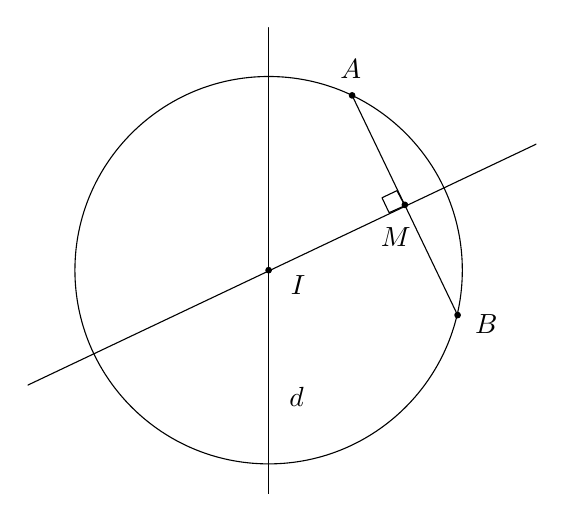
\begin{tikzpicture}[line cap=round,line join=round,>=stealth,x=1.0cm,y=1.0cm]
\clip(1.24,-1.) rectangle (7.7,4.92);
\draw (5.93,2.85) -- (5.74,2.76) -- (5.83,2.57) -- (6.03,2.66) -- cycle;
\draw (4.3,1.84) circle (2.46cm);
\draw (5.36,4.06)-- (6.7,1.27);
\draw [domain=1.24:7.7] plot(\x,{(-0.36--0.82*\x)/1.73});
\draw (4.3,-1.) -- (4.3,4.92);
\draw (5.6,4.4) node[left] {$A$};
\draw (6.8,1.4) node[anchor=north west] {$B$};
\draw (5.6,2.5) node[anchor=north west] {$M$};
\draw (4.44,0.48) node[anchor=north west] {$d$};
\draw (4.46,1.9) node[anchor=north west] {$I$};
\draw [fill=black] (4.3,1.84) circle (1.0pt);
\draw [fill=black] (5.36,4.06) circle (1.0pt);
\draw [fill=black] (6.7,1.27) circle (1.0pt);
\draw [fill=black] (6.03,2.67) circle (1.0pt);
\end{tikzpicture}
}
}
\end{ex}

\begin{ex}%[Dự án C THPTQG 2025]%[Vương Quốc Phong]%[0D0C2-6]
Một bàn cờ vua gồm $8 \times 8$ ô vuông, mỗi ô có cạnh bằng $1$ đơn vị. Một ô vừa là hình vuông hay hình chữ nhật, hai ô là hình chữ nhật, \ldots. Có bao nhiêu cách họn ngẫu nhiên một hình vuông có cạnh lớn hơn $4$ đơn vị.
% \shortans{437}
\loigiai{
Ta coi bàn cờ vua được xác định bởi $9$ đường thẳng theo phương nằm ngang $x=0$; $x=1$;$x=2$;\ldots;$x=8$.
và $9$ đường thẳng theo phương thẳng đứng $y=0$; $y=1$; $y=2$;\ldots; $y=8$. \\
% Mỗi hình chữ nhật được tạo thành từ hai đoạn thẳng thuộc hai đường thẳng $x_i$, $x_j$ và hai đoạn thẳng thuộc các đường thẳng $y_m$, $y_n$ ($i, j, m, n \in \left\{0;2;3;4;5;6;7;8\right\}$) nên có $C_9^2 \cdot C_9^2$ hình chữ nhật. \\ Suy ra số hình chữ nhật tạo thành là $C_9^2 \cdot C_9^2 \Rightarrow n\left(\Omega \right)=C_9^2 \cdot C_9^2=1296$. \\
% Gọi $A$ là biến cố hình được chọn là hình vuông có cạnh $a$ lớn hơn $4$.
\begin{itemize}
\item  Trường hợp 1: $a=5$. Khi đó mỗi hình vuông được tạo thành do hai đường thẳng $x_i$, $ x_j$ cách nhau $5$ đơn vị và hai đường thẳng $y_m$, $y_n$ cách nhau $5$ đơn vị nên có $4\cdot 4=16$ cách chọn.
\item  Trường hợp 2: $a=6$. Khi đó mỗi hình vuông được tạo thành do hai đường thẳng $x_i$, $ x_j$ cách nhau $6$ đơn vị và hai đường thẳng $y_m$, $y_n$ cách nhau $6$ đơn vị có $3 \cdot 3=9$ cách chọn.
\item Trường hợp 3: $a=7$. Khi đó mỗi hình vuông được tạo thành do hai đường thẳng $x_i$, $ x_j$ cách nhau $7$ đơn vị và hai đường thẳng $y_m$, $ y_n$ cách nhau $7$ đơn vị có $2 \cdot 2=4$ cách chọn.
\item  Trường hợp 4: $a=8$. Khi đó mỗi hình vuông được tạo thành do hai đường thẳng $x_i$, $x_j$ cách nhau $8$ đơn vị và hai đường thẳng $y_m$, $y_n$ cách nhau $8$ đơn vị nên có $1 \cdot 1=1$ cách chọn.
\end{itemize}
Suy ra $n(A)=14+9+4+1=30$. \\
% Xác suất để hình được chọn là một hình vuông có cạnh lớn hơn $4$ đơn vị là \[P(A) = \dfrac{n(A)}{n(\Omega)} = \dfrac{30}{1296} = \dfrac{5}{216}.\] \\
% Suy ra $ a = 5; b = 216 \Rightarrow a + 2b = 437$.
}
\end{ex}
\Closesolutionfile{ans}
\Closesolutionfile{ansbook}
